
%% The Appendices part is started with the command \appendix;
%% appendix sections are then done as normal sections
\appendix

\section{Magnetic Field Gradient Calculations}
\label{Appendix:MagneticFieldGradientCalculations}

The maximum gradient in the z-component of the magnetic field in Figure~\ref{fig:bfield_1gironeffects} was calculated by taking the difference between the maximum and the minumum magnetic-field magnitudes along the perimeter of the PMT outline (in this case in the diagonal direction), and dividing it by the distance between the two points of measurement (here, the diameter of the PMT, 20 inches = 0.508 m).
For the first plot, without any GIRON flooring, the gradient is calculated as follows:
\[[(-223\pm5 mG) - (-447\pm5 mG)]/0.508 m\]
\[=(224\pm5 mG)/0.508 m\]
\[=(224 mG \pm 2.23\%)/0.508 m\]
\[=441 mG/m \pm 2.23\%\]
\[=440 \pm 10 mG/m \]
Similarly, the gradient for the second plot, with one layer of GIRON flooring is calculated to be $ 160 \pm 10 mG/m $.

The percent difference between the magnetic-field gradient with and without GIRON flooring is:
\[(160\pm10 mG/m - 440\pm10 mG/m)/(440\pm10 mG/m)\]
\[=-63\pm7\%\]

Therefore, a single layer of GIRON flooring helps reduce the gradient in the z-component of the magnetic field by $ 63\pm7\% $.

\section{Magnetic Field Compensation Coil Configuration}
\label{Appendix:CoilPositions}
%
\begin{figure}[h]
  \begin{center}
  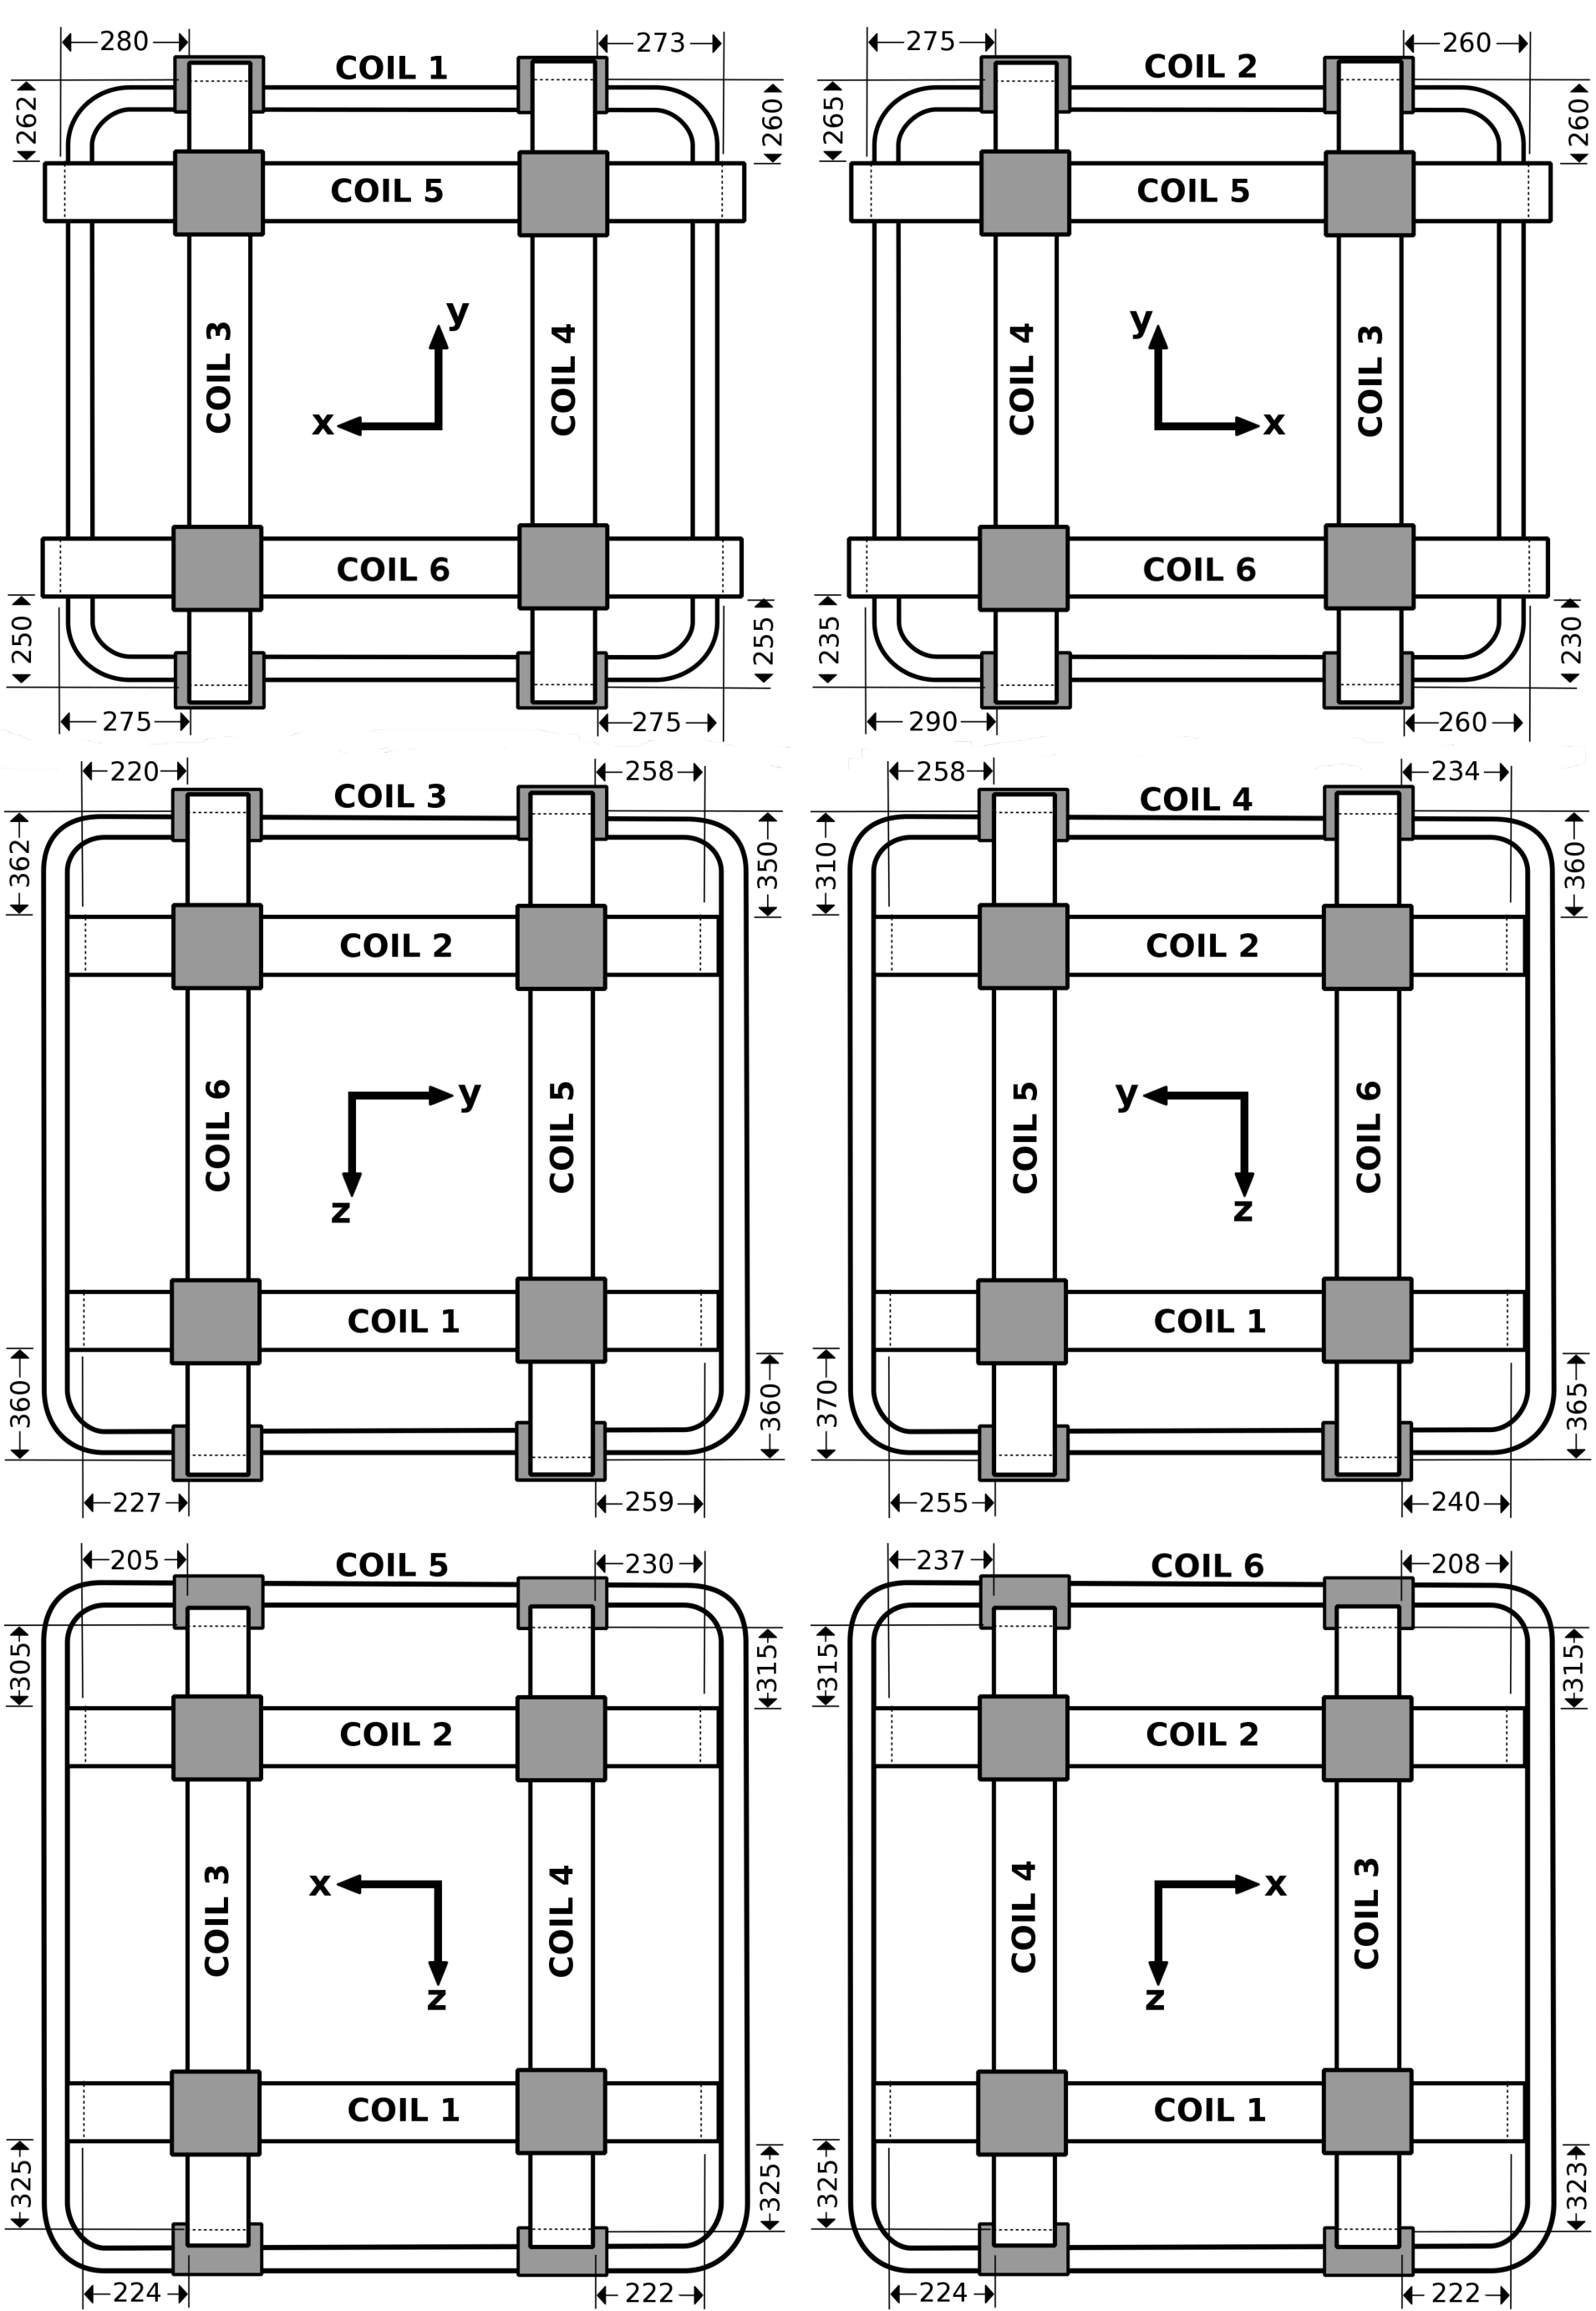
\includegraphics[width=0.8\textwidth]{bfield_PTFcoilpositions.pdf}
  \caption{PTF compensation coil positions; dimensions are in millimeters ($\pm2$mm).}
  \label{fig:coils}
  \end{center}
\end{figure}
%
